\red{Fill this part out with all the stuff that is and isnt tangible that you’ve been doing (Matt)}

\subsection{Object Detection}
In order for the aircraft to safely navigate while searching for Joe, it must first know where it is safe to move in the environment. State-of-the-art autonomous vehicles commonly use Red-Green-Blue-Depth cameras, allowing them to get both visual and depth/distance information simultaneously; while these cameras are powerful, they are also expensive. Instead, a low-cost option combining data from the camera and LiDAR sensors shown in Section \ref{sec:sensing} was chosen to approximate an RGB-D camera.\\

Object detection is initiated once the aircraft reaches the remote landing site. Figure \ref{fig:scan} shows the progression of data acquisition using the LiDAR.\\

Elaborate:
\begin{itemize}
	\item Initially empty occupancy map (Figure \ref{fig:scaninit})
	\item LiDAR identifies distances from aircraft, which are converted to ``occupied'' cells/voxels in the map (Figure \ref{fig:scanten})
	\item Once a reasonable amount of data has been acquired (Figure \ref{fig:scanminute}), the map is filtered to eliminate ``isolated'' voxels
	\item The resulting map is then grouped into ``supervoxels'', large areas that the aircraft cannot traverse
\end{itemize}

\subsection{Path Planning}
\red{Planning module takes the occupancy grid, then generates a flight path the aircraft can traverse. Rescanning is performed if the aircraft moves out of the ``known'' area.}

\begin{figure}
	\centering
	\begin{subfigure}[b]{0.55\textwidth}
		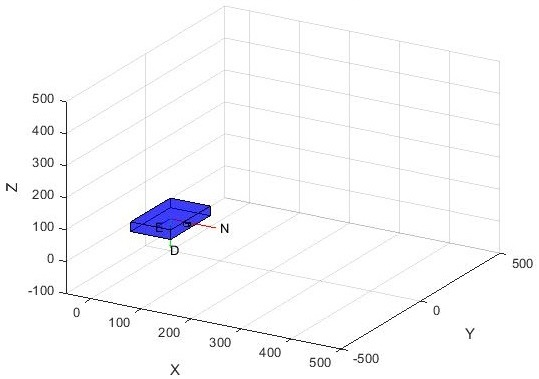
\includegraphics[width=\textwidth]{\IMAGEPATH Data/voxelize0s}
		\caption{Initial (empty) environment}
		\label{fig:scaninit}
	\end{subfigure}
	
	\begin{subfigure}[b]{0.55\textwidth}
		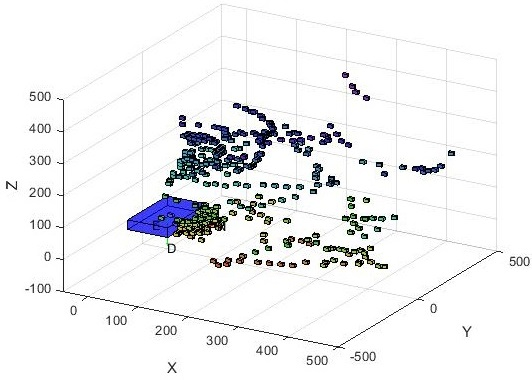
\includegraphics[width=\textwidth]{\IMAGEPATH Data/voxelize10s}
		\caption{10s of data acquisition}
		\label{fig:scanten}
	\end{subfigure}
	
	\begin{subfigure}[b]{0.55\textwidth}
		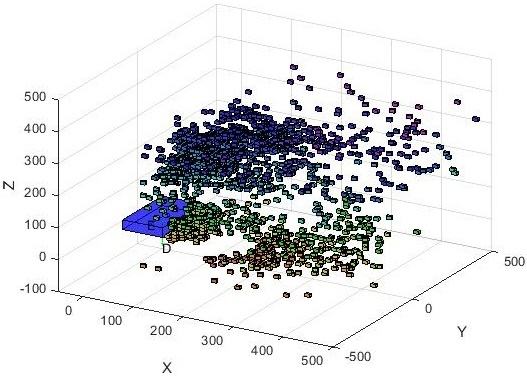
\includegraphics[width=\textwidth]{\IMAGEPATH Data/voxelize60s}
		\caption{60s of data acquisition}
		\label{fig:scanminute}
	\end{subfigure}
	\caption{Scanning the environment with the LiDAR}
	\label{fig:scan}
\end{figure}